\documentclass[12pt]{article}

\usepackage[margin=0.85in]{geometry}
\usepackage{amsmath, amsthm, amssymb}
\usepackage{enumerate}
\usepackage[utf8]{inputenc}
\usepackage{xcolor}
\usepackage{graphicx}
\usepackage{caption}
\usepackage{listings}
\lstset{
  basicstyle=\ttfamily\tiny
}


\begin{document}

\title{Linear Least Squares}
\author{John DeSilva}

\maketitle

\section*{Introduction}
This project dealt with determining a quadratic least squares approximation for
the flight of a tennis ball, given an overdetermined system consisting of the
approximate position of the ball during its flight. This fit could then be used
to determine if the tennis ball fell `in' or `out', allowing players to
challenge calls. The positions were approximated using a number of cameras, and
the given dataset contained 101 coordinates in the $X, Z$ plane. With this
data, I used the Scala programming language along with the Breeze library to
compute a fit, and plot the figures.  Breeze aims to be matlab-like, so I was
able to create, transpose, and multiply vectors and matrices with ease.
\section*{Quadratic Fit}
It was given that the dataset was an approximation of a quadratic function of
the form $c_1 x^2 + c_2 x + c_3$, and upon viewing the plotted data, it was
clear that a parabola would be a good fit. To compute my fit, I solved the
normal equation, $A^TAx^{*} = A^Tb$ for $x^{*}$. In this case $A^TA$ is
invertible, the equation can be rearranged as $x^{*} = (A^TA)^{-1}A^Tb$ which is
readily solved by Breeze. But what are $A$ and $b$ in this situation? It is
clear that $b$ is simply the $Z$ coordinate data that we are attempting to fit a
line to. It is a column vector of size 101 by 1. A is created using our $X$
coordinate data, but is modified in such a way that we are solving for the three
constants $c_1, c_2, \text{ and } c_3$. For each data point in the $X$
coordinate data, we have a row of three elements $c_1 * x^2, c_2 * x, \text{ and
} c_3$. The normal equation minimizes the error created at each point, which is
the error between our approximation function $f(x) = c_1 x^2 + c_2 x + c_3$, a
row of $A$, and the actual point, a row of $b$. Upon solving the normal
equation, I determined $x^{*}$ to be
\begin{align*}
  [-0.017989293972666846, 0.19015793929643401, 2.9979685010321635]
\end{align*}
so that $c_1 \approx -0.018, c_2 \approx 0.190, \text{ and } c_3 \approx 3.00$.
The data points and the fit are shown in Figure 1. These coefficients are
consistent with the plot; the parabola is upside down (negative $c_1$) and it
has a $Z$ intercept of about $3$ feet ($c_3$). This means that our function is
\begin{equation*}
  f^{*}(x) = -0.0179\ldots x^2 + 0.190\ldots x + 2.997\ldots
\end{equation*}
Upon inspecting the graph, it is 
clear that the ball is `in', because its $Z$ coordinate is less than 0 before
reaching $X = 78$ feet.
\begin{figure}[p]
  \centering
  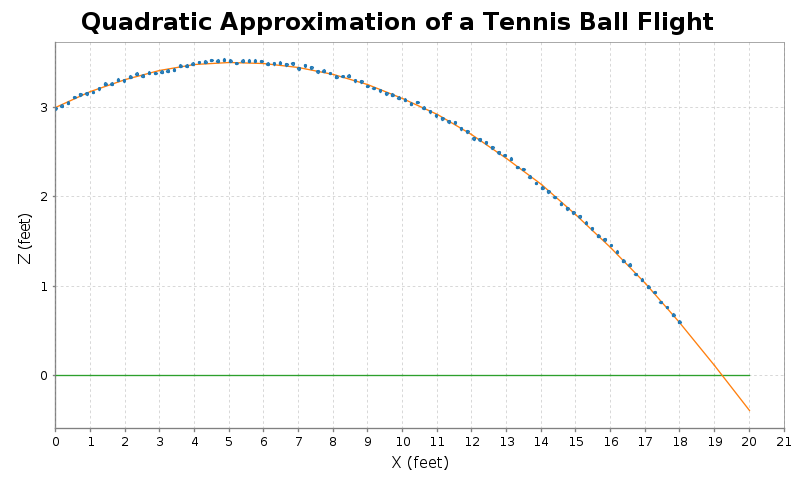
\includegraphics[width=0.8\textwidth]{fit.png}
  \caption{}
\end{figure}\\
\section*{Error}
The error of our fit can be analyzed as a function of $N$, the number of data
points (in this case camera shots) used to fit our function. The error as a
function of $N$ is given by
\begin{equation*}
  e = \frac{1}{N} \sqrt{\sum_{i = 0}^{N} [f^{*}(x_i) - z_i ]^2 }
\end{equation*}
and is computed by computing the $f^{*}$ fit function with $N$ data points. The
function $f^{*}$ applied to the domain of $X$ coordinates is denoted $z*$, the
approximate $Z$ coordinates. The sum of squares portion of the error can be
computed like the following in Scala: 
\begin{verbatim} 
(zStar.take(n), z.take(n)).zipped.map(_-_).map(_*_).map(_+_)
\end{verbatim}
This takes the first $n$ elements of $z^{*}$ and $z$, and makes one list from
two by combining them pairwise. Next, it maps `subtraction' onto each pair, then
takes each element from the resulting list and multiplies it by itself, and then
folds the list left by adding each element to its neighbor until there is only
one element.  Finally, the error can be computed by taking the square root of
this result and dividing by $N$. Figure 2 shows how the average error decreases
as more samples are taken. To reach our target error of $3.0 \times 10^{-3}$
feet ($\approx 1$mm, the horizontal line on the plot) we need at least 32
samples (the vertical line on the plot).
\begin{figure}[p]
  \centering
  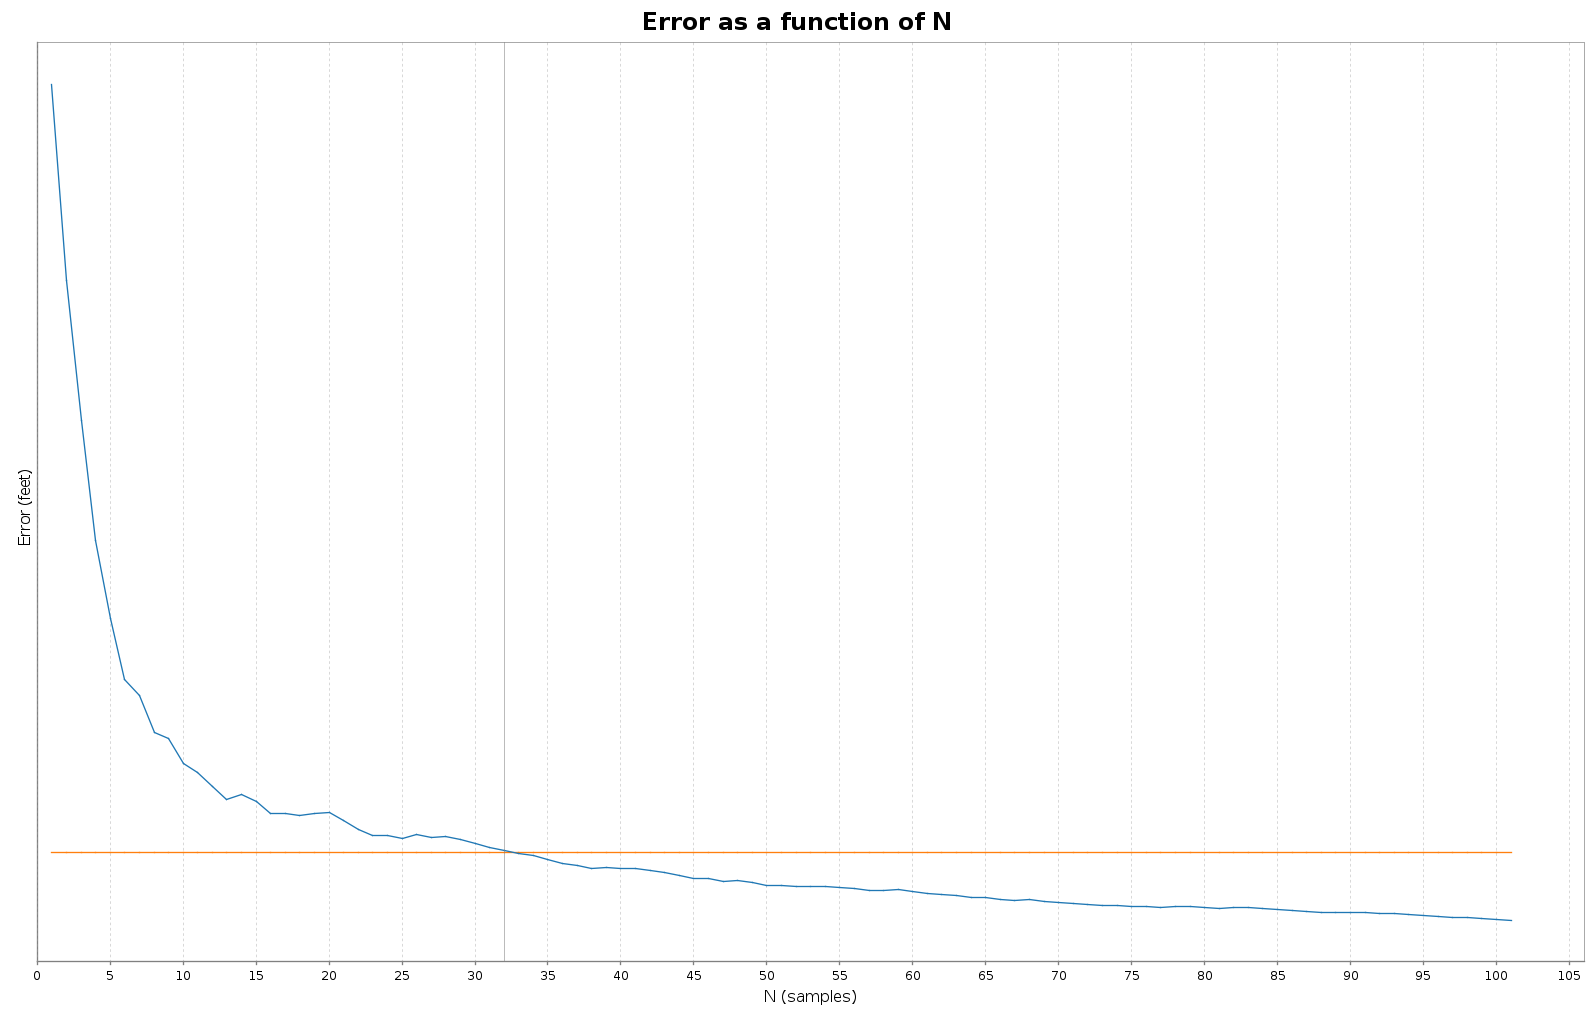
\includegraphics[width=0.8\textwidth]{error.png}
  \caption{}
\end{figure}\\

\newpage
\lstinputlisting[language=Java]{../src/LeastSquares.scala}

\end{document}
